\documentclass{beamer}
%\documentclass[handout]{beamer} %Use the handout version to suppress the overlays

% Specify a theme.  There are tons to choose from!
\usetheme{Boadilla}
\setbeamertemplate{footline}
{
  \leavevmode%
  \hbox{%
  \begin{beamercolorbox}[wd=.4\paperwidth,ht=2.25ex,dp=1ex,center]{title in head/foot}%
    \usebeamerfont{title in head/foot}\insertshorttitle
  \end{beamercolorbox}%
  \begin{beamercolorbox}[wd=.5\paperwidth,ht=2.25ex,dp=1ex,center]{author in head/foot}%
    \usebeamerfont{author in head/foot}\hspace*{3em}\insertsection\hspace*{3em}
  \end{beamercolorbox}%
  \begin{beamercolorbox}[wd=.1\paperwidth,ht=2.25ex,dp=1ex,right]{title in head/foot}%
    \usebeamerfont{title in head/foot}\insertframenumber{} / \inserttotalframenumber\hspace*{2ex}
  \end{beamercolorbox}}%
  \vskip0pt%
}
\makeatletter
\setbeamertemplate{navigation symbols}{}



% This makes the grayed out text for overlays
\setbeamercovered{transparent}

% Load packages:
\usepackage{amsfonts, amsmath, amsthm, amssymb}
\usepackage{listings} %for inserting code
\usepackage{tikz}
\usepackage{pgfplots}
\usepackage{physics}
\usepackage{amsmath}
\DeclareMathOperator*{\argmin}{arg\,min}

\usepackage{multibib}
% Define new citation commands
\newcites{frameone}{References}
\newcites{frametwo}{Acknowledgements}


% My Shortcuts:
\newcommand{\ds}{\displaystyle}
\newsavebox{\codebox}% For storing listings



% Title page details:
\title{Explicit Non-Linear Dimensionality Reduction}
\author{Pierre Visconti}
\institute{Department of Mathematics, Walla Walla University}
\date{03 May 2024}

% Content:
\begin{document}

\begin{frame}	
\titlepage
\end{frame}

\begin{frame}{Outline}
	\tableofcontents
\end{frame}



\section[Introduction]{Introduction and Motivation}

\begin{frame}{Complexity of Datasets in Machine Learning}
        \begin{figure}
    		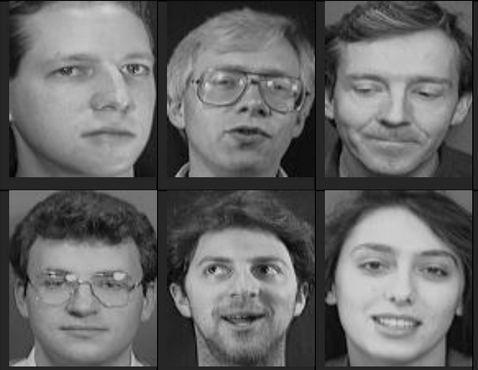
\includegraphics[,width=8cm]{images/face.png}
    		%\caption{Swissroll - 2000 observations.}
        \end{figure}
\end{frame}

\begin{frame}{Complexity of Datasets in Machine Learning}
        \begin{block}{Image size}
        Each image: 200x300 pixels = 60,000 pixels per image.
        \end{block}
        \begin{tabular}{|c|c|c|c|c|}
        \hline
        \textbf{Image ID} & \textbf{Pixel 0} & \textbf{Pixel 1} & \textbf{...} & \textbf{Pixel (59,999)} \\
        \hline
        Img\_00 & 120 & 135 & ... & 90 \\
        \hline
        Img\_01 & 100 & 110 & ... & 95 \\
        \hline
        Img\_02 & 130 & 125 & ... & 85 \\
        \hline
        ... & ... & ... & ... & ... \\
        \hline
        Img\_n-1 & 115 & 105 & ... & 100 \\
        \hline
        \end{tabular}
       \pause
        \begin{block}{Time complexity}
        Number of operations.
        \begin{itemize}
        \item Decision Trees: O($mn\log{(n)}$)
        \item Naive Bayes: $\text{O}(mn)$
        \end{itemize}
        \end{block}
\end{frame}

\begin{frame}{Complexity of Datasets in Machine Learning}
        \begin{figure}
    		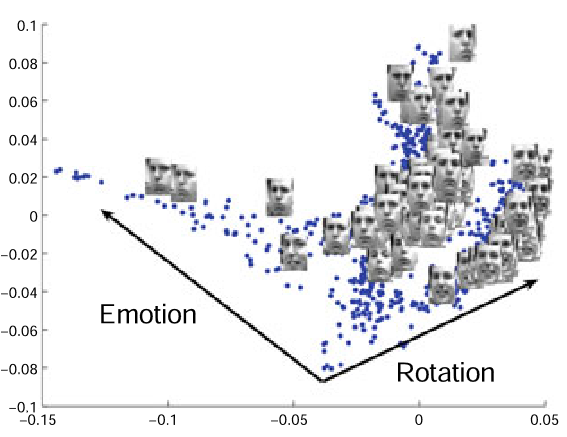
\includegraphics[,width=8cm]{images/faces.png}
    		%\caption{Swissroll - 2000 observations.}
        \end{figure}
\end{frame}

\begin{frame}{Dimensionality Reduction}
\begin{block}{}
    Dimensionality reduction is the act of reducing high dimensional data to a lower dimension while retaining the intrinsic properties of the data. 
\end{block}
\pause
\begin{block}{Issues with current algorithms}
    \begin{itemize}[<+->]
    \item  Linear techniques such as Principal Components Analysis (PCA) cannot handle complex non-linear data. 
    \item Manifold Learning algorithms, can handle non-linear data, however most existing algorithms assume a linear mapping and do not produce an explicit model.
    \item Goal:
    \begin{itemize}
        \item Explore a manifold learning algorithm that produces an explicit non-linear model.  
    \end{itemize}
    \end{itemize}
\end{block}
\end{frame}

\begin{frame}{Importance of Producing an Explicit Model}
\begin{figure}
    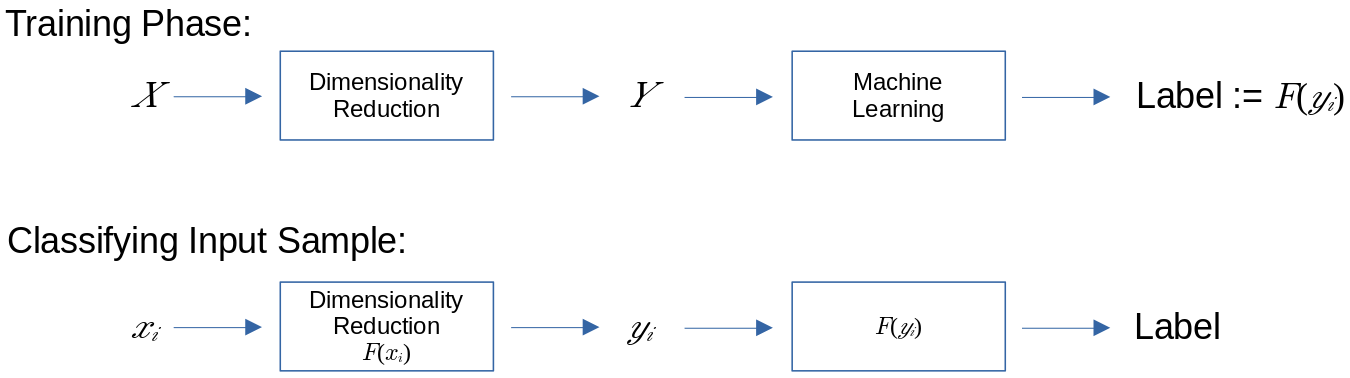
\includegraphics[,width=12cm]{images/explicit_model.png}
    %\caption{Swissroll - 2000 observations.}
\end{figure}
\pause
\begin{block}{Explicit}
\begin{itemize}
    \item Closed form expression.
    \item Independent of training samples.
\end{itemize}
\end{block}
\end{frame}

\section[Mathematical Intuition]{Mathematical Intuition}
\begin{frame}{Outline}
    \tableofcontents[current]
\end{frame}

\begin{frame}{Manifolds and Embeddings}
\begin{block}{Definition: smooth manifold}
$M$ is a smooth manifold of dimension $d$ if it is a topological space where, 
\begin{itemize}
    \item For every $p,q \in M$ there exists disjoint open subsets $U,V \subseteq M$, such that $p \in U$ and $q \in V$.
    \item There exists a countable basis for the topology of $M$.
    \item For every $p \in M$, there exists
    \begin{itemize}
        \item an open subset $U \subseteq M$ containing p,
        \item an open subset $\hat{U} \subseteq \mathbf{R}^d$, and
        \item a homeomorphism $\phi: U \rightarrow \hat{U}$
    \end{itemize}
\end{itemize}
\end{block}
\pause
\begin{block}{}
    A topological space that that has a differentiable structure and locally resembles Euclidean space near every point. The dimension $d$ is called the intrinsic dimension. 
\end{block}
\end{frame}

\begin{frame}{Manifolds and Embeddings}
\begin{block}{Definition: embedding}
A smooth map between two manifolds whose inverse exists and is also smooth. 
\begin{itemize}
    \item Maps elements from one space to another.
\end{itemize}
\end{block}
\pause
\begin{block}{Properties of embeddings}
    \begin{itemize}
        \item Injective
        \item Preserves the structure of the object being embedded.
        \item Manifold learning:
        \begin{itemize}
            \item The points close to each other in the high dimensional space remain close in the low dimensional space. 
        \end{itemize}
    \end{itemize}
\end{block}
\end{frame}

\begin{frame}{The Manifold Assumption and Manifold Learning}
\begin{block}{The manifold assumption}
    The data is sampled from a distribution that is close to or supported on, a smooth manifold of dimension $d$, embedded in $\mathbf{R}^n$. 
\end{block}
\pause
\begin{block}{Application to manifold learning}
\begin{itemize}[<+->]
    \item The manifold learning algorithm finds a mapping $F$ of a high dimensional point in $\mathbf{R}^n$, to a lower dimensional point in $\mathbf{R}^m$, denoted $\mathbf{R}^n \rightarrow \mathbf{R}^m$.
    \item Assume that $n > d$.
    \item Desire that $n > m$ and $m \geq d$. 
    \item Desire that the embedding is found explicitly and is non-linear in nature.
    \begin{itemize}
        \item "Explore a manifold learning algorithm that produces an explicit non-linear model."
    \end{itemize}
\end{itemize}
\end{block}
\end{frame}




\section[Developing an Algorithm]{Developing an Algorithm}
\begin{frame}{Outline}
\tableofcontents[current]
\end{frame}

\begin{frame}{Locally Linear Embedding (LLE)}
LLE aims to preserve local relationships between data points.
\begin{block}{First Step}
\begin{itemize}[<+->]
    \item Find the linear coefficients that best reconstructs each data point $x_i$ by its $k$-nearest neighbors. 
    \item Using Euclidean Distance, the linear reconstruction weights $R_{ij}, i,j=1,2,...,N$ are given by minimizing the sum of the squared distances between all the data points and their reconstructions.
    \begin{itemize}
        \item $x_i$ is only reconstructed from its neighbors
        \item the weights for $x_i$ must sum to 1. 
    \end{itemize}
\end{itemize}
\pause
\[R_{ij} = \argmin_{\sum_{j=1}^N{R_{ij}}=1}\quad\sum_{i=1}^N{\norm{x_i - \sum_{j=1}^N{R_{ij}x_j}}}_{2}^2 \tag{i}\]
\end{block}    
\end{frame}


\begin{frame}{Locally Linear Embedding}
\begin{block}{Second Step}
    \par LLE then constructs an embedding using the weights $R$, while optimizing the coordinates $y_i$, to minimize the error.
    \begin{itemize}
        \item Unit Covariance
        \item Zero Mean
    \end{itemize}
\begin{align*}
    \min{} \quad &\sum_{i=1}^N{\norm{y_i-\sum_{j=1}^N{R_{ij}y_j}}_2^2} \tag{ii}\\
    \\
    \text{s.t.} \quad &\frac{1}{N}\sum_{i=1}^N{y_iy_i^T=I_m} \\
    & \sum_{i=0}^{N}{y_i}=0
\end{align*}
\end{block}
\end{frame}


\begin{frame}[fragile]{Polynomial Mapping Assumption} % fragile frame is required for verbatim text.  
    \par Given a data set $\mathcal{X}:=\{x_1, x_2, ..., x_N\}$ in the high dimensional space $\mathbf{R} ^n$, assume there exists an explicit polynomial mapping from $\mathcal{X}$ to its low dimensional representation $\mathcal{Y}:=\{y_1, y_2, ..., y_N\}$ in $\mathbf{R}^m$. 
    \\ 
    \pause
    \begin{block}{}The $k$-th component of $y_i \in \mathcal{Y}$ is defined as a polynomial of degree $p$ with respect to $x_i$, such that
    \[y_{i}^{(k)} = v_k^T\phi(x_i), \text{ where } v_k \in \mathbf{R}^{pn}\]
    \end{block}
    \pause
    \begin{block}{Mapping function $\phi(x)$}
    For a given data vector $x_i \in \mathcal{X}$, define the mapping $\phi:\mathbf{R}^n\rightarrow\mathbf{R}^{pn}$ as
    \[\phi(x_i) =
    \begin{bmatrix}
    \overbrace{x_i \odot x_i \odot \cdots \odot x_i}^{p \text{ times}} \\
    \vdots \\
    x_i \odot x_i \\
    x_i
    \end{bmatrix}.\]
    \end{block}
\end{frame}

\section{NPPE Algorithm}
\begin{frame}{Outline}
\tableofcontents[current]
\end{frame}
\begin{frame}{NPPE Algorithm Overview}
\par \textbf{Neighborhood Preserving Polynomial Embedding (NPPE)}
\par Given a data set $\mathcal{X}:=\{x_1, x_2, ..., x_N\}$ in the high dimensional space $\mathbf{R} ^n$, the NPPE algorithm finds an explicit polynomial mapping from $\mathcal{X}$ to its low dimensional representation $\mathcal{Y}:=\{y_1, y_2, ..., y_N\}$ in $\mathbf{R}^m$.
\vspace{0.5cm}
\pause
\begin{block}{NPPE Algorithm}
\par \textbf{Inputs:} Data matrix $X=[x_1 \hspace{0.5cm} x_2 \text{ }\cdots\text{ } x_N]$ of size $n \times N$, the number $k$ of nearest neighbors, the polynomial degree $p$, and the low dimensional space $m$. 
\pause
\begin{enumerate}
\item Compute the linear weights $R$.
\item Compute the non-linear weights $W$.
\item Solve the generalized eigenvalue problem to get the eigenvectors $v_i, i=1,2,...,m$.
\item Map the high-dimensional data to the low-dimensional embedding space.
\end{enumerate}
\end{block}
\end{frame}

\begin{frame}{NPPE Algorithm - Step 1}
\begin{block}{Computing the Linear Weights}
\[R_{ij} = \argmin_{\sum_{j=1}^N{R_{ij}}=1}\quad\sum_{i=1}^N{\norm{x_i - \sum_{j=1}^N{R_{ij}x_j}}}_{2}^2 \tag{i}\]
The linear weight matrix $R=\left[r_1 \hspace{0.5cm} r_2 \text{ }\cdots\text{ } r_N\right]$ in $\mathbf{R}^{N \times N}$, is given by computing the following closed formed solution for $r_i$, where 
\begin{itemize}
    \item $e$ is a column vector of all ones 
    \item $G_{jl}=(x_j-x_i)^T(x_l-x_i)$ where $x_j,\,x_l$ are in the $k$-nearest neighbors of $x_i$. 
\end{itemize}
\begin{equation}
r_i = \frac{G^{-1}e}{e^TG^{-1}e}
\end{equation}
\end{block}
\end{frame}

\begin{frame}{NPPE Algorithm - Step 2}
\begin{block}{Computing the Non-linear Weights}
The non-linear weight matrix $W\in\mathbf{R}^{N\times N}$, is computed by the following equation. 
\begin{equation}
W_{ij} = R_{ij} + R_{ji} - \sum_{k=1}^{N}{R_{ik}R_{kj} \text{, and } \sum_{j=1}^N{W_{ij}}=1}
\end{equation}
\end{block}
\end{frame}

\begin{frame}{NPPE Algorithm - Step 3}
\begin{block}{LLE Eigenvalue Problem}
\begin{itemize}[<+->]
    \item Define an eigenvalue problem as $Av=\lambda v$.
    \[A = (I-R)^T(I-R)\]
\end{itemize}
\end{block}
\pause
\begin{block}{Solving the Generalized Eigenvalue Problem for NPPE}
\begin{itemize}
    \item Define a generalized eigenvalue problem as $Av=\lambda Bv$.
\end{itemize}
\pause
\begin{equation}
\phi(D-W)\phi^Tv_i = \lambda \phi D\phi^Tv_i, \quad v_i^T\phi D\phi^Tv_j=\delta_{ij}
\end{equation}
\begin{itemize}[<+->]
    \item Define $\phi = \left[\phi(x_1) \hspace{0.5cm} \phi(x_2) \text{ }\cdots\text{ } \phi(x_N)\right]$ to be a $(pn) \times N$ matrix.
     \item The optimal solutions are found by obtaining the eigenvectors $v_i, i=1,2,...,m$, corresponding to the $m$ smallest eigenvalues.
\end{itemize}
\end{block}
\end{frame}

\begin{frame}{NPPE Algorithm - Step 4}
\begin{block}{Polynomial Mapping Assumption}
    \[y_{i}^{(k)} = v_k^T\phi(x_i), \text{ where } v_k \in \mathbf{R}^{pn}\]
\end{block}
\pause 
\begin{block}{Mapping to the Low Dimensional Space}
For a data sample $x_i \in \mathcal{X}$, its low dimensional representation $y_i \in \mathcal{Y}$ is given by
\begin{equation}
y_i = \left[ v_1^T\phi(x_i) \hspace{0.5cm} v_2^T\phi(x_i) \text{ }\cdots\text{ } v_m^T\phi(x_i)  \right]^T
\end{equation}
Importantly, the mapping function above holds true for a new data sample $x_t \notin \mathcal{X}$, allowing for its low dimensional representation $y_t$ to be computed efficiently. 
\end{block}
\end{frame}




\section{Results and Conclusion}
\begin{frame}{Outline}
\tableofcontents[current]
\end{frame}
\begin{frame}{Results on Swissroll Dataset}
    The parameter of $k$-nearest neighbors is set to be $1\%$ of the training samples $N$ and the polynomial degree $p=2$.    \vspace{1cm} 
    \begin{columns} % Start the columns environment
        \begin{column}{.5\textwidth} % Begin the first column
            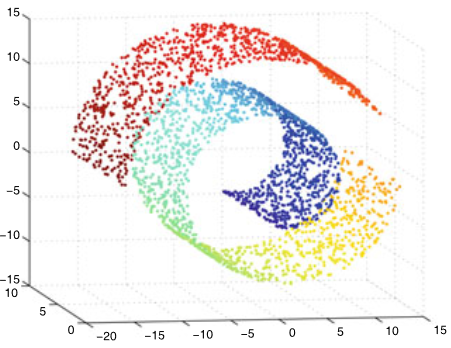
\includegraphics[width=0.8\linewidth]{images/hd.png}
            \caption{SwissRoll dataset in $\mathbf{R}^3$}
        \end{column}
        \begin{column}{.5\textwidth} % Begin the second column
            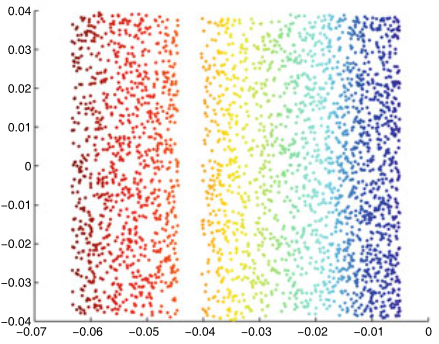
\includegraphics[width=0.8\linewidth]{images/ld.png}
            \caption{SwissRoll representation in $\mathbf{R}^2$}
        \end{column}
    \end{columns}
\end{frame}

\begin{frame}{My Current Results}
    \begin{columns} % Start the columns environment
        \begin{column}{.5\textwidth} % Begin the first column
            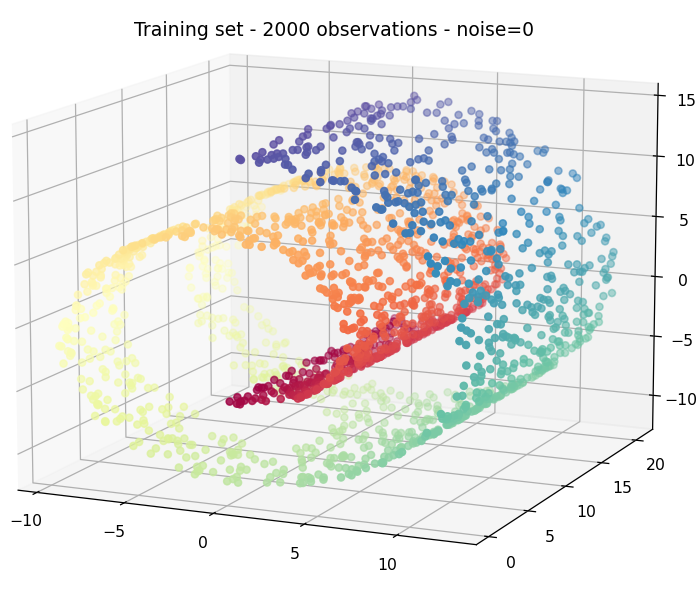
\includegraphics[width=1\linewidth]{images/train_h.png}
            %\caption{SwissRoll dataset in $\mathbf{R}^3$}
        \end{column}
        \begin{column}{.5\textwidth} % Begin the second column
            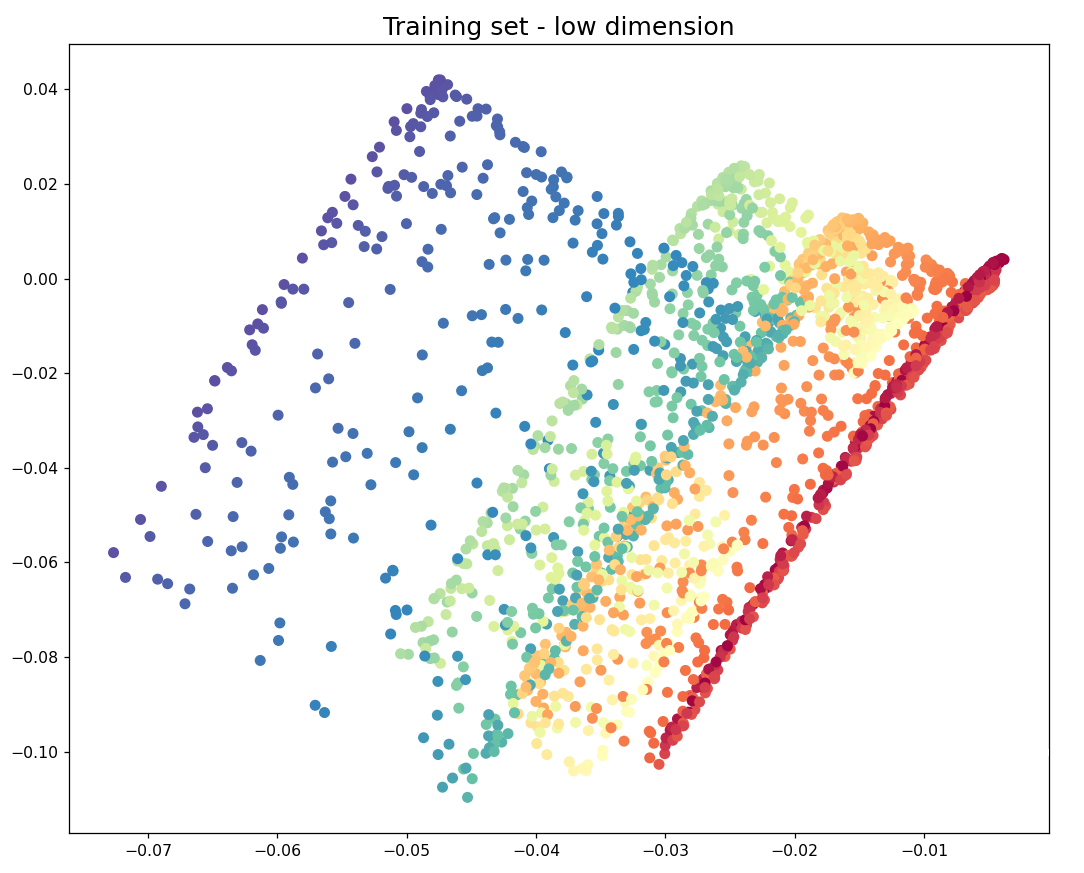
\includegraphics[width=1\linewidth]{images/train_l.png}
            %\caption{SwissRoll representation in $\mathbf{R}^2$}
        \end{column}
    \end{columns}
\end{frame}

\begin{frame}{Performance on New Data}
    \begin{columns} % Start the columns environment
        \begin{column}{.5\textwidth} % Begin the first column
            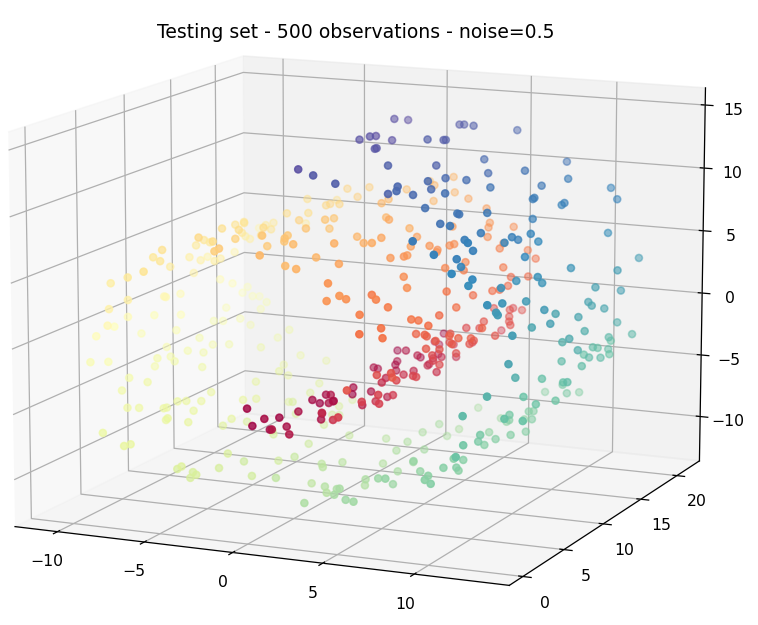
\includegraphics[width=1\linewidth]{images/test_h.png}
            %\caption{SwissRoll dataset in $\mathbf{R}^3$}
        \end{column}
        \begin{column}{.5\textwidth} % Begin the second column
            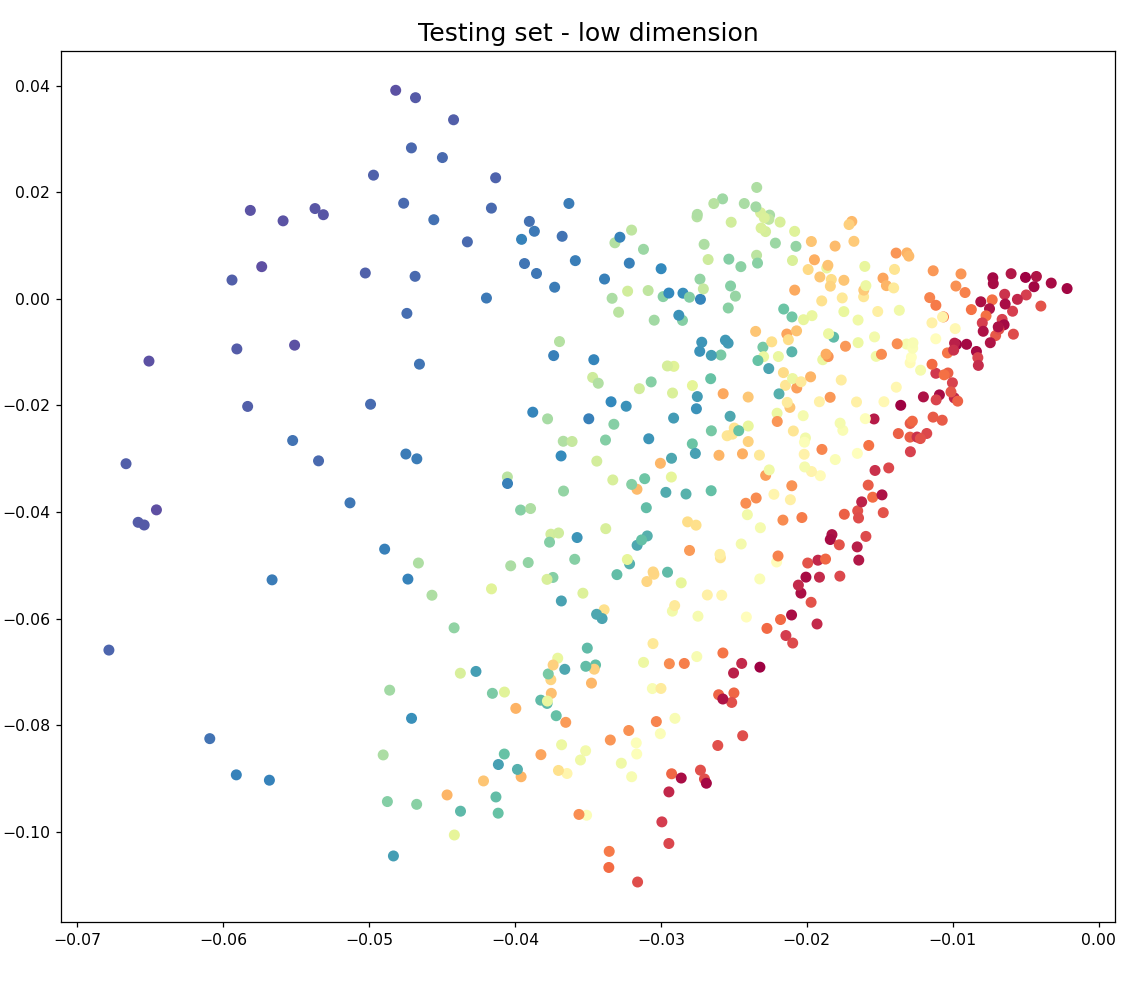
\includegraphics[width=1\linewidth]{images/test_l.png}
            %\caption{SwissRoll representation in $\mathbf{R}^2$}
        \end{column}
    \end{columns}
\end{frame}

\begin{frame}{Future Work}
    \begin{block}{}
    \begin{itemize}[<+->]
        \setlength\itemsep{1em}
        \item Use the algorithm as a pre-processing step to improve the performance of machine learning algorithms.
        \item Improving the algorithm to use less memory / GPU Compute.
        \item Research methods for estimating the intrinsic dimension.
        \item Applications in image/data compression.
    \end{itemize}
    \end{block}
\end{frame}

% First frame with its own bibliography
\begin{frame}[allowframebreaks]{References}
    \fontsize{6}{12}\selectfont
    \nociteframeone{*}
    \bibliographystyleframeone{plain}
    \bibliographyframeone{refs} % Entries are in the refs.bib file
\end{frame}

% Second frame with its own bibliography
\begin{frame}{Acknowledgements}
    \fontsize{6}{10}
    \text{Research Advisor: Jonathan Duncan, PhD}
    \vspace*{1cm}
    \fontsize{6}{12}
    \nociteframetwo{*}
    \bibliographystyleframetwo{plain}
    \bibliographyframetwo{acks} % Entries are in the acks.bib file
\end{frame}

\begin{frame}{Questions?}
\end{frame}

\end{document}



